\documentclass{article}
\usepackage{fontspec}
\usepackage{xeCJK}
%\usepackage[xetex]{graphicx}

\usepackage{titlesec}
\usepackage{verbatim}
%provides multi-line comment syntax : \begin{comment} \end{comment}
%provides href/url
\usepackage{hyperref}
\usepackage{cleveref}

\title{NASA hw6}
\author{B04902045 孫凡耘}
\date{\today}

\begin{document}
\maketitle
    \section{Network Administration}
    \subsection{1}
    \subsubsection{a}
    Generally Speaking, the primary differences between the two frequencies are the range (coverage) and bandwidth (speed) that the bands provide. The 2.4 GHz band provides coverage at a longer range but transmits data at slower speeds. The 5 GHz band provides less coverage but transmits data at faster speeds.\newline
    In my own words:5G 頻段開放的比較較多,標準比較新,支持的帶寬也很高,利用不同的調變與多工技術能使數位訊號具有更高的資料傳輸率(資訊攜載量與其頻寬有直接的相關)。
    \subsubsection{b}
    No ! \newline
    1.理論上 5G 的訊號衰減比較快,所以多數情形下會得到比 2.4G 弱的訊號,訊號太弱 就會得到慢一些的速度。看這張圖就算蠻清楚的,距離遠(或通過牆壁之類的介質)時2.4G的data transfer rate就很有可能比5G還要好。
     \begin{figure}[!htb]
            \begin{flushleft}
            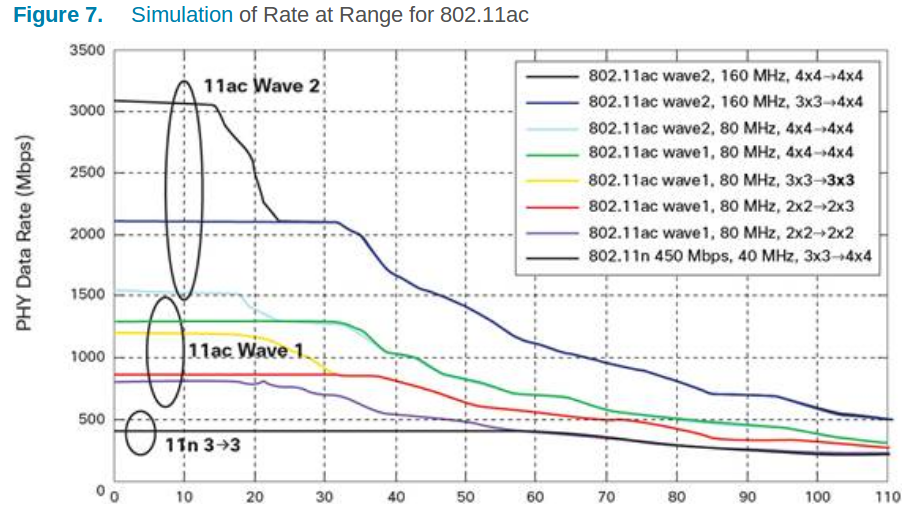
\includegraphics[scale=0.25]{pic.png}
            \end{flushleft}
    \end{figure}
    reference: \url{http://www.cisco.com/c/en/us/products/collateral/wireless/aironet-3600-series/white_paper_c11-713103.html#_Toc383047849}\newline
    2. 當然資料傳輸率也跟頻段的密度有關,如果某個地方2.4G的裝置很少反而5G的裝置很多也有可能導致2.4G比較快。(雖然現在幾乎不太有這種情形
    \subsection{2}

    \subsubsection{a}
Use the following command, it prints out all details of access points nearby
\begin{verbatim}
$ sudo iwlist wlan0 scan
\end{verbatim}
    Answer: WPA2
    \subsubsection{b}
    The most significant changes between WPA and WPA2\newline
    1. the mandatory use of AES algorithms \newline
    2. the introduction of CCMP (Counter Cipher Mode with Block Chaining Message Authentication Code Protocol) as a replacement for TKIP (still preserved in WPA2 as a fallback system and for interoperability with WPA).
    \subsubsection{c}
    \textbf{WEP}\newline
    disadvantage
    \begin{itemize}
        \item WEP encryption uses a shared key authentication and sends the same key with data packets being transmitted across the wireless network. If malicious users have enough time and gather enough data they can eventually piece together their own key.
        \item if the master key needs to be changed, it will have to be manually changed on all devices connected to the network. This can be a tedious task if you have many devices connected to your network.
    \end{itemize}
    advantage
    \begin{itemize}
        \item When users happen to see your network during wireless detection, they will most likely be discouraged since it will require a key. This makes it clear to the user that they are not welcome.
        \item  WEP offers is interoperability, since all wireless devices support basic WEP encryption. This can be useful when trying to use older devices that need wireless connectivity.
    \end{itemize}
    \textbf{WPA2}\newline
    disadvantage
    \begin{itemize}
        \item being incompatibility with legacy hardware and older operating systems.
        \item larger performance overhead and increases data packet size leading to longer transmission. More processing power needed.
    \end{itemize}
    advantage
    \begin{itemize}
        \item WPA2 addresses this problem with the introduction of the AES algorithm. Theoretically, passphrases created with the AES algorithm are virtually uncrackable.
         \item  dynamic encryption keys
    \end{itemize}


    \begin{comment}
    \begin{itemize}
        \item
        \item
        \item
        \item
    \end{itemize}
    $ dx = [0, -1, 1, 0] $\newline\newline
    $ dy = [1, 0, 0, -1] $\newline\newline
    $ E_{i,j} = 1 + \sum_{dir=0}^{3} p_{dir}*(E_{i+dx[dir],j+dy[dir]} \quad \textrm{if} \quad available(i+dx[dir],j+dy[dir])\quad \textrm{else}\quad E_{i,j} )$
    \newline\newline
    $ \sum_{i=0}^{3} P_{i} = 1 $\newline\newline
    $ H_{4}^{10} - 4 = 282 $
    \newline
    \end{comment}
\end{document}
